% !TEX TS-program = pdflatex
\documentclass[11pt]{article}

% -------------------- Packages --------------------
\usepackage[a4paper,margin=1in]{geometry}
\usepackage{amsmath,amssymb}
\usepackage[T1]{fontenc}
\usepackage{lmodern}
\usepackage{xcolor}
\usepackage{tcolorbox}
\tcbuselibrary{skins,breakable}
\usepackage{enumitem}
\usepackage{hyperref}
\usepackage{tikz}
\usetikzlibrary{calc,angles,quotes}

\pagestyle{empty}

% -------------------- Dark Theme Colors --------------------
\definecolor{bg}{HTML}{000000}
\definecolor{pairbg}{HTML}{121212}
\definecolor{solbg}{HTML}{0A0A0A}
\definecolor{border}{HTML}{2A2A2A}
\definecolor{text}{HTML}{FFFFFF}
\definecolor{muted}{HTML}{C9CDD3}
\definecolor{gold}{HTML}{FFD700}
\definecolor{green}{HTML}{4ADE80}
\definecolor{cyan}{HTML}{38BDF8}

\pagecolor{bg}
\color{text}

\hypersetup{
  colorlinks=true,
  linkcolor=cyan,
  urlcolor=cyan
}

\setlength{\parindent}{0pt}
\setlength{\parskip}{10pt}

\setlist[itemize]{left=1.4em,itemsep=6pt,topsep=6pt}
\setlist[enumerate]{left=1.6em,itemsep=4pt,topsep=4pt}

% -------------------- tcolorbox Base --------------------
\tcbset{
  enhanced,
  breakable,
  arc=12pt,
  boxrule=0.8pt,
  left=16pt,right=16pt,top=12pt,bottom=12pt
}

\newtcolorbox{QAPair}[1]{%
  colback=pairbg,
  colbacklower=solbg,
  colframe=border,
  coltext=text,
  title=\textcolor{gold}{\bfseries #1},
  fonttitle=\bfseries,
  coltitle=text,
  segmentation style={draw=border, dashed, line width=0.6pt},
}

% Visible text inside this box (fix)
\newtcolorbox{QuickBox}{%
  colback=pairbg,
  colframe=cyan,
  coltext=text,
  fontupper=\color{text},
  borderline north={4pt}{0pt}{cyan},
  arc=14pt,
  boxrule=0.8pt
}

% Helper for step headings
\newcommand{\Step}[1]{\textcolor{muted}{\textbf{Step #1:}}}

% -------------------- TikZ styles --------------------
\tikzset{
  geom/.style={draw=cyan, line width=0.9pt, line cap=round, line join=round},
  thickgeom/.style={draw=cyan, line width=1.2pt, line cap=round, line join=round},
  guide/.style={draw=muted, line width=0.7pt, dashed},
  pt/.style={circle, fill=green, inner sep=1.7pt},
  lab/.style={text=text},
}

% ============================================================
\begin{document}

\begin{center}
{\LARGE\bfseries \textcolor{gold}{Exercise 9.7 --- Solutions}}\\[-2pt]
\end{center}

\begin{QuickBox}
{\color{cyan}\bfseries Quick facts about loci (very useful)}\par\medskip
\begin{itemize}
\item \textbf{Points at a fixed distance from a point $O$} form a \textbf{circle} with centre $O$.
\item \textbf{Points equidistant from two points $X$ and $Y$} lie on the \textbf{perpendicular bisector} of $\overline{XY}$.
\item \textbf{Points at a fixed distance from a line $l$} form \textbf{two lines parallel} to $l$ (one on each side).
\item \textbf{Points equidistant from two intersecting lines} lie on the \textbf{angle bisectors} (internal and external).
\item In an \textbf{equilateral triangle}, \textbf{circumcenter = incenter = centroid = orthocenter} (all coincide).
\end{itemize}
\end{QuickBox}

% ============================================================
% Q1
\begin{QAPair}{Question 1}
\textcolor{gold}{\bfseries Question:} Draw $AB=6$ cm. Bisect $AB$ at $O$ and draw the locus of point $P$ equidistant from $O$ and above $AB$. What is the name of the locus?\\
\tcblower
\textcolor{green}{\bfseries Answer:}
\[
\begin{aligned}
\Step{1}\;& \text{All points at a fixed distance from }O\text{ form a circle with centre }O.\\
\Step{2}\;& \text{Because we want the points \emph{above }AB\text{, the locus is the \textbf{upper semicircle}.}}
\end{aligned}
\]
\textbf{Name of locus:} \textbf{Semicircle (part of a circle)} with centre $O$ (above $AB$).

\medskip
\begin{center}
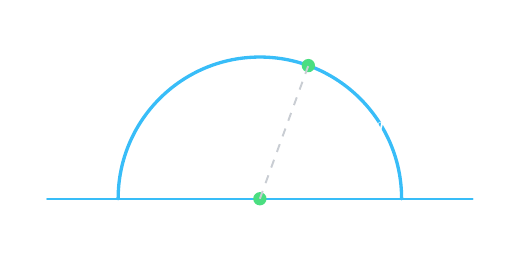
\begin{tikzpicture}[scale=0.9]
  \coordinate (A) at (0,0);
  \coordinate (B) at (6,0);
  \coordinate (O) at (3,0);

  \draw[geom] (A)--(B);
  \node[lab, below] at (A) {$A$};
  \node[lab, below] at (B) {$B$};
  \node[pt] at (O) {};
  \node[lab, below] at (O) {$O$};

  % upper semicircle (example radius)
  \draw[thickgeom] ($(O)+(2,0)$) arc (0:180:2);
  \coordinate (P) at ($(O)+(70:2)$);
  \node[pt] at (P) {};
  \node[lab, above right] at (P) {$P$};
  \draw[guide] (O)--(P);
  \node[lab, right] at ($(O)!0.55!(P)$) {$OP=r$};
\end{tikzpicture}
\end{center}
\end{QAPair}

% ============================================================
% Q2
\begin{QAPair}{Question 2}
\textcolor{gold}{\bfseries Question:} Draw coordinate axes. Take $A$ on $x$-axis and $B$ on $y$-axis at a distance of $4.5$ cm each from origin. Draw the locus of points from $A$ to $B$ equidistant from origin. Name this locus. How many such loci can be drawn around the origin?\\
\tcblower
\textcolor{green}{\bfseries Answer:}
\[
\begin{aligned}
\Step{1}\;& OA=OB=4.5\text{ cm, so both }A\text{ and }B\text{ lie on a circle centred at }O.\\
\Step{2}\;& \text{The locus of points equidistant from }O\text{ (with distance }4.5\text{ cm) is that circle.}\\
\Step{3}\;& \text{``From }A\text{ to }B\text{'' gives the \textbf{arc }AB\text{, i.e. a \textbf{quarter circle (quadrant)}.}}
\end{aligned}
\]
\textbf{Name:} \textbf{Quadrant (quarter of a circle)} of radius $4.5$ cm with centre at origin.

\textbf{How many around the origin?} \textbf{Four quadrants} (one in each quadrant of the coordinate plane).

\medskip
\begin{center}
\begin{tikzpicture}[scale=0.85]
  \coordinate (O) at (0,0);
  \coordinate (A) at (4.5,0);
  \coordinate (B) at (0,4.5);

  \draw[geom,->] (-0.5,0)--(5.2,0) node[lab, right] {$x$};
  \draw[geom,->] (0,-0.5)--(0,5.2) node[lab, above] {$y$};

  \node[pt] at (O) {}; \node[lab, below left] at (O) {$O$};
  \node[pt] at (A) {}; \node[lab, below] at (A) {$A$};
  \node[pt] at (B) {}; \node[lab, left]  at (B) {$B$};

  \draw[guide] (O)--(A) node[midway, below] {$4.5$};
  \draw[guide] (O)--(B) node[midway, left] {$4.5$};

  \draw[geom] (O) circle (4.5);
  \draw[thickgeom] (A) arc (0:90:4.5); % arc from A to B
\end{tikzpicture}
\end{center}
\end{QAPair}

% ============================================================
% Q3
\begin{QAPair}{Question 3}
\textcolor{gold}{\bfseries Question:} Draw a horizontal line $l$.
\begin{enumerate}
\item[(i)] Take a point $T$ above $l$ at a distance $3$ cm and draw a locus through $T$ parallel to $l$.
\item[(ii)] Take a point $Q$ below $l$ at a distance $3.2$ cm and draw a locus through $Q$ parallel to $l$.
\item[(iii)] What is the distance between both loci?
\end{enumerate}
\tcblower
\textcolor{green}{\bfseries Answer:}
\[
\begin{aligned}
\Step{1}\;& \text{(i) The locus through }T\text{ parallel to }l\text{ is a \textbf{line} }l_1\parallel l.\\
\Step{2}\;& \text{(ii) The locus through }Q\text{ parallel to }l\text{ is a \textbf{line} }l_2\parallel l.\\
\Step{3}\;& \text{(iii) Since }T\text{ is }3\text{ cm above }l\text{ and }Q\text{ is }3.2\text{ cm below }l,\\
& \qquad \text{distance between }l_1\text{ and }l_2 = 3+3.2 = \boxed{6.2\text{ cm}}.
\end{aligned}
\]

\medskip
\begin{center}
\begin{tikzpicture}[scale=0.9]
  \draw[geom] (-4,0)--(4,0);
  \node[lab, right] at (4,0) {$l$};

  \coordinate (T) at (0,3);
  \coordinate (Q) at (1,-3.2);

  \draw[thickgeom] (-4,3)--(4,3);
  \node[lab, right] at (4,3) {$l_1$};

  \draw[thickgeom] (-4,-3.2)--(4,-3.2);
  \node[lab, right] at (4,-3.2) {$l_2$};

  \node[pt] at (T) {}; \node[lab, above] at (T) {$T$};
  \node[pt] at (Q) {}; \node[lab, below] at (Q) {$Q$};

  \draw[guide] (-3.2,0)--(-3.2,3) node[midway, left] {$3$ cm};
  \draw[guide] (-2.7,0)--(-2.7,-3.2) node[midway, left] {$3.2$ cm};
  \draw[guide,<->] (3.4,3)--(3.4,-3.2) node[midway, right] {$6.2$ cm};
\end{tikzpicture}
\end{center}
\end{QAPair}

% ============================================================
% Q4
\begin{QAPair}{Question 4}
\textcolor{gold}{\bfseries Question:} A circle has centre $P$. $X$ and $Y$ are on the circumference.
\begin{enumerate}
\item[(i)] Draw locus of points equidistant from $X$ and $Y$ through $P$.
\item[(ii)] Take another point $Z$ on the locus outside the circle and draw another circle of radius $PZ$.
\item[(iii)] What is the relation of this circle with the given circle?
\end{enumerate}
\tcblower
\textcolor{green}{\bfseries Answer:}
\[
\begin{aligned}
\Step{1}\;& \text{(i) Points equidistant from }X\text{ and }Y\text{ lie on the \textbf{perpendicular bisector} of }XY.\\
\Step{2}\;& \text{Since }PX=PY\text{ (radii), }P\text{ lies on that perpendicular bisector, so the locus passes through }P.\\
\Step{3}\;& \text{(ii) Choose }Z\text{ on this perpendicular bisector (outside the first circle) and draw a circle centred at }P\\
&\qquad \text{with radius }PZ.\\
\Step{4}\;& \text{(iii) Both circles have the \textbf{same centre }P\text{, hence they are \textbf{concentric circles}.}}
\end{aligned}
\]

\medskip
\begin{center}
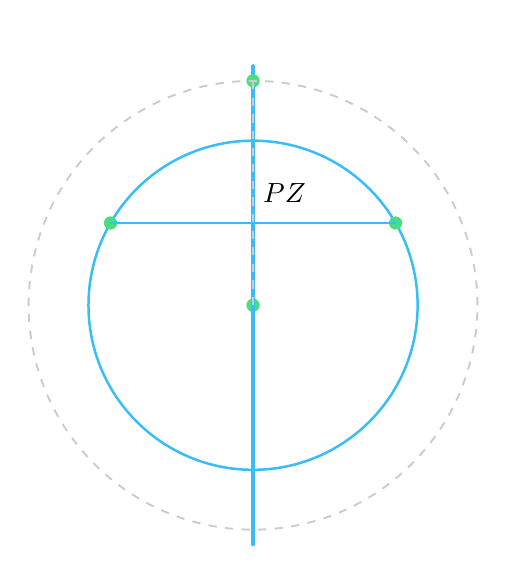
\begin{tikzpicture}[scale=0.95]
  \coordinate (P) at (0,0);
  \coordinate (X) at ($(P)+(30:2.2)$);
  \coordinate (Y) at ($(P)+(150:2.2)$);

  \draw[geom] (P) circle (2.2);
  \node[pt] at (P) {}; \node[lab, below right] at (P) {$P$};

  \node[pt] at (X) {}; \node[lab, above right] at (X) {$X$};
  \node[pt] at (Y) {}; \node[lab, above left]  at (Y) {$Y$};

  \draw[geom] (X)--(Y); % chord XY

  % Perpendicular bisector through P (since chord is symmetric here)
  \draw[thickgeom] (0,-3.2)--(0,3.2);
  \node[lab, above] at (0,3.2) {locus};

  \coordinate (Z) at (0,3.0);
  \node[pt] at (Z) {}; \node[lab, right] at (Z) {$Z$};

  \draw[guide] (P)--(Z) node[midway, right] {$PZ$};

  % New larger circle (concentric)
  \draw[guide] (P) circle (3.0);
\end{tikzpicture}
\end{center}
\end{QAPair}

% ============================================================
% Q5
\begin{QAPair}{Question 5}
\textcolor{gold}{\bfseries Question:} Draw a line $AB$. Let $P$ and $Q$ be two points not on $AB$ but coplanar with $AB$. Draw the locus of points from $P$ to $Q$.
\begin{enumerate}
\item[(i)] What is the name of that locus?
\item[(ii)] Is there any point on the locus $PQ$ (if extended) which lies on line $AB$?
\item[(iii)] How can we take points $P$ and $Q$ such that no point of the locus lies on line $AB$?
\item[(iv)] How can we take $P$ and $Q$ such that every point of line $AB$ may lie on the locus?
\end{enumerate}
\tcblower
\textcolor{green}{\bfseries Answer:}
\[
\begin{aligned}
\Step{1}\;& \text{(i) The locus from }P\text{ to }Q\text{ is the \textbf{line segment }PQ\text{ (a straight line).}}\\
\Step{2}\;& \text{(ii) If the straight line }PQ\text{ (extended) intersects }AB,\text{ then there is \textbf{one} common point.}\\
&\qquad \text{If }PQ\parallel AB,\text{ then there is \textbf{no} common point.}\\
\Step{3}\;& \text{(iii) To ensure \textbf{no point} of the locus lies on }AB,\text{ choose }PQ\parallel AB.\\
\Step{4}\;& \text{(iv) To make \textbf{every point} of line }AB\text{ lie on the locus, take }P\text{ and }Q\text{ \textbf{on }AB}\\
&\qquad \text{(so the locus line }PQ\text{ coincides with }AB\text{).}
\end{aligned}
\]

\medskip
\begin{center}
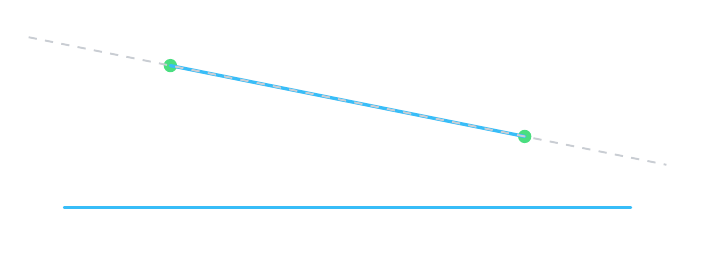
\begin{tikzpicture}[scale=0.9]
  \draw[geom] (-4,0)--(4,0);
  \node[lab, right] at (4,0) {$AB$};

  \coordinate (P) at (-2.5,2.0);
  \coordinate (Q) at (2.5,1.0);

  \node[pt] at (P) {}; \node[lab, above] at (P) {$P$};
  \node[pt] at (Q) {}; \node[lab, above] at (Q) {$Q$};

  \draw[thickgeom] (P)--(Q);
  \node[lab, above right] at ($(P)!0.55!(Q)$) {locus $PQ$};

  % show extension meeting AB
  \draw[guide] ($(P)!-0.4!(Q)$)--($(P)!1.4!(Q)$);
\end{tikzpicture}
\end{center}
\end{QAPair}

% ============================================================
% Q6
\begin{QAPair}{Question 6}
\textcolor{gold}{\bfseries Question:} Draw an equilateral triangle $PQR$.
\begin{enumerate}
\item[(i)] Draw right bisectors of any two sides and locate point $A$ where both meet.
\item[(ii)] Draw angle bisectors of any two vertices and locate point $B$ where both meet.
\item[(iii)] What is the relation between locus of $A$ and $B$?
\end{enumerate}
\tcblower
\textcolor{green}{\bfseries Answer:}
\[
\begin{aligned}
\Step{1}\;& \text{(i) The perpendicular bisectors meet at the \textbf{circumcenter} }A.\\
\Step{2}\;& \text{(ii) The angle bisectors meet at the \textbf{incenter} }B.\\
\Step{3}\;& \text{(iii) In an \textbf{equilateral} triangle, circumcenter and incenter are the \textbf{same point}.}\\
&\qquad \Rightarrow \boxed{A \equiv B\ \text{(they coincide).}}
\end{aligned}
\]

\medskip
\begin{center}
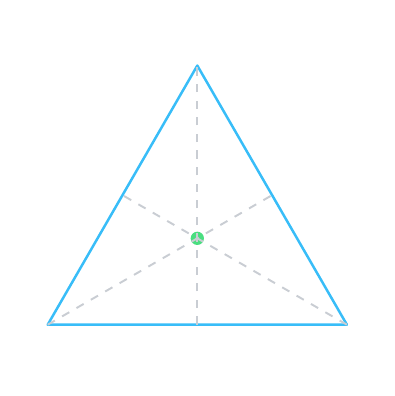
\begin{tikzpicture}[scale=0.95]
  \coordinate (P) at (-2,0);
  \coordinate (Q) at (2,0);
  \coordinate (R) at (0,3.464);

  \draw[geom] (P)--(Q)--(R)--cycle;
  \node[lab, below] at (P) {$P$};
  \node[lab, below] at (Q) {$Q$};
  \node[lab, above] at (R) {$R$};

  % "center" (exact centroid)
  \coordinate (C) at (barycentric cs:P=1,Q=1,R=1);
  \node[pt] at (C) {};
  \node[lab, right] at (C) {$A=B$};

  % a couple of bisectors (schematic)
  \draw[guide] ($(P)!0.5!(Q)$)--(R);
  \draw[guide] (P)--($(Q)!0.5!(R)$);
  \draw[guide] (Q)--($(P)!0.5!(R)$);
\end{tikzpicture}
\end{center}
\end{QAPair}

% ============================================================
% Q7
\begin{QAPair}{Question 7}
\textcolor{gold}{\bfseries Question:} The figure shows an isosceles triangle $ABC$ with $AB=AC$. Prove that the locus (line) of the bisector of $\angle A$ is the right (perpendicular) bisector of side $BC$.\\
\tcblower
\textcolor{green}{\bfseries Answer (proof):}
Let $AD$ be the bisector of $\angle A$ meeting $BC$ at $D$.
\[
\begin{aligned}
\Step{1}\;& AB=AC \qquad (\text{given})\\
\Step{2}\;& AD=AD \qquad (\text{common side})\\
\Step{3}\;& \angle BAD = \angle DAC \qquad (\text{since }AD\text{ bisects }\angle A)
\end{aligned}
\]
So $\triangle ABD \cong \triangle ACD$ by \textbf{SAS}.
\[
\begin{aligned}
\Step{4}\;& \Rightarrow BD=DC \qquad (\text{corresponding parts})\\
\Step{5}\;& \Rightarrow \angle ADB = \angle ADC \qquad (\text{corresponding parts})
\end{aligned}
\]
But $B,D,C$ are collinear, so $\angle ADB+\angle ADC=180^\circ$.  
If they are equal, each is $90^\circ$, hence $AD\perp BC$.

Therefore, $AD$ is \textbf{perpendicular} to $BC$ and also \textbf{bisects} $BC$:
\[
\boxed{AD\text{ is the perpendicular (right) bisector of }BC.}
\]

\medskip
\begin{center}
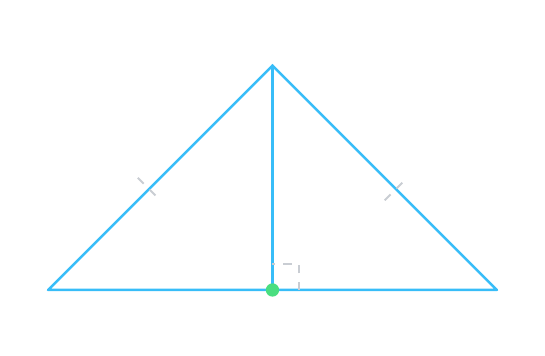
\begin{tikzpicture}[scale=0.95]
  \coordinate (B) at (-3,0);
  \coordinate (C) at (3,0);
  \coordinate (A) at (0,3);
  \coordinate (D) at (0,0);

  \draw[geom] (A)--(B)--(C)--cycle;
  \draw[thickgeom] (A)--(D);

  \node[lab, above] at (A) {$A$};
  \node[lab, below] at (B) {$B$};
  \node[lab, below] at (C) {$C$};
  \node[pt] at (D) {}; \node[lab, below] at (D) {$D$};

  % marks AB=AC (schematic)
  \draw[guide] ($(A)!0.55!(B)$) ++(-0.15,0.15)--++(0.3,-0.3);
  \draw[guide] ($(A)!0.55!(C)$) ++(-0.15,-0.15)--++(0.3,0.3);

  % right angle mark at D
  \draw[guide] (D) ++(0.35,0) -- ++(0,0.35) -- ++(-0.35,0.0);
\end{tikzpicture}
\end{center}
\end{QAPair}

% ============================================================
% Q8
\begin{QAPair}{Question 8}
\textcolor{gold}{\bfseries Question:} Draw three non-collinear points in a plane. Find the locus of the points which are equidistant from these three points. How many such points exist?\\
\tcblower
\textcolor{green}{\bfseries Answer:}
\[
\begin{aligned}
\Step{1}\;& \text{Three non-collinear points form a triangle.}\\
\Step{2}\;& \text{Points equidistant from two vertices lie on the perpendicular bisector of their segment.}\\
\Step{3}\;& \text{The point equidistant from \emph{all three} vertices is the intersection of perpendicular bisectors.}
\end{aligned}
\]
So the required point is the \textbf{circumcenter} of the triangle.

\[
\boxed{\text{Exactly one such point exists (unique circumcenter).}}
\]

\medskip
\begin{center}
\begin{tikzpicture}[scale=0.95]
  \coordinate (A) at (-2,0.5);
  \coordinate (B) at (2,0);
  \coordinate (C) at (0,3);

  \draw[geom] (A)--(B)--(C)--cycle;
  \node[lab, left]  at (A) {$A$};
  \node[lab, right] at (B) {$B$};
  \node[lab, above] at (C) {$C$};

  % perpendicular bisectors (schematic)
  \coordinate (Mab) at ($(A)!0.5!(B)$);
  \coordinate (Mbc) at ($(B)!0.5!(C)$);

  \draw[guide] ($(Mab)+(-0.2,2.4)$)--($(Mab)+(0.2,-2.4)$);
  \draw[guide] ($(Mbc)+(-2.2,1.2)$)--($(Mbc)+(2.2,-1.2)$);

  % circumcenter (approx)
  \coordinate (O) at (0.1,1.25);
  \node[pt] at (O) {};
  \node[lab, right] at (O) {circumcenter};

\end{tikzpicture}
\end{center}
\end{QAPair}

% ============================================================
% Q9
\begin{QAPair}{Question 9}
\textcolor{gold}{\bfseries Question:} Take two lines $AB$ and $CD$ inclined at $60^\circ$ intersecting at $O$.
\begin{enumerate}
\item[(i)] Draw locus of points equidistant from both lines.
\item[(ii)] Draw bisector of $60^\circ$.
\item[(iii)] What is the relation between locus of points equidistant from lines and angle bisector?
\item[(iv)] Draw bisector of adjacent angle at $O$ and find relation between both angle bisectors.
\end{enumerate}
\tcblower
\textcolor{green}{\bfseries Answer:}
\[
\begin{aligned}
\Step{1}\;& \text{(i) Points equidistant from two intersecting lines lie on the \textbf{angle bisectors}.}\\
&\qquad \text{So the locus consists of \textbf{two lines}: the \textbf{internal} and \textbf{external} bisectors.}\\
\Step{2}\;& \text{(ii) The bisector of }60^\circ\text{ is the \textbf{internal} angle bisector making }30^\circ\text{ with each line.}\\
\Step{3}\;& \text{(iii) Therefore, the locus of points equidistant from the lines is \textbf{exactly the angle bisectors}.}\\
\Step{4}\;& \text{(iv) The adjacent angle is }120^\circ;\ \text{its bisector is another line.}\\
&\qquad \text{The bisectors of supplementary angles are \textbf{perpendicular}. Hence the two bisectors meet at }90^\circ.
\end{aligned}
\]
\[
\boxed{\text{Internal and external angle bisectors are perpendicular to each other.}}
\]

\medskip
\begin{center}
\begin{tikzpicture}[scale=0.95]
  \coordinate (O) at (0,0);

  % two lines forming 60 degrees
  \draw[geom] (-4,0)--(4,0); % AB (horizontal)
  \draw[geom] (0,0)--(60:4);  % CD ray
  \draw[geom] (0,0)--(240:4); % opposite ray

  \node[pt] at (O) {}; \node[lab, below left] at (O) {$O$};

  % internal bisector at 30 degrees
  \draw[thickgeom] (0,0)--(30:4);
  \node[lab, above right] at (30:3.6) {bisector of $60^\circ$};

  % external bisector (bisector of 120 degrees): perpendicular to internal
  \draw[thickgeom] (0,0)--(120:4);
  \node[lab, above left] at (120:3.5) {bisector of $120^\circ$};

  % angle marking (schematic)
  \draw[guide] (1.3,0) arc (0:60:1.3);
  \node[lab] at (35:1.7) {$60^\circ$};
\end{tikzpicture}
\end{center}
\end{QAPair}

\end{document}